

\section{Introduction}


Video inpainting aims to recover the missing content of a corrupted video and assist lots of practical applications, e.g., video restoration and watermarking removal. 
High-quality video inpainting requires not only realistic structures with visual details but also temporal consistency. 
Compared with image inpainting, video inpainting is significantly more challenging due to the extra time dimension, while human eyes are sensitive to flickers and jitters.
% 
Though great progress has been made in 2D image inpainting using deep learning techniques \cite{yu2018free,Xiong_2019_CVPR}, directly applying these approaches to each frame individually for video inpainting will lead to flaws, flickers and jitters. 

\begin{figure}[t]
	\centering
	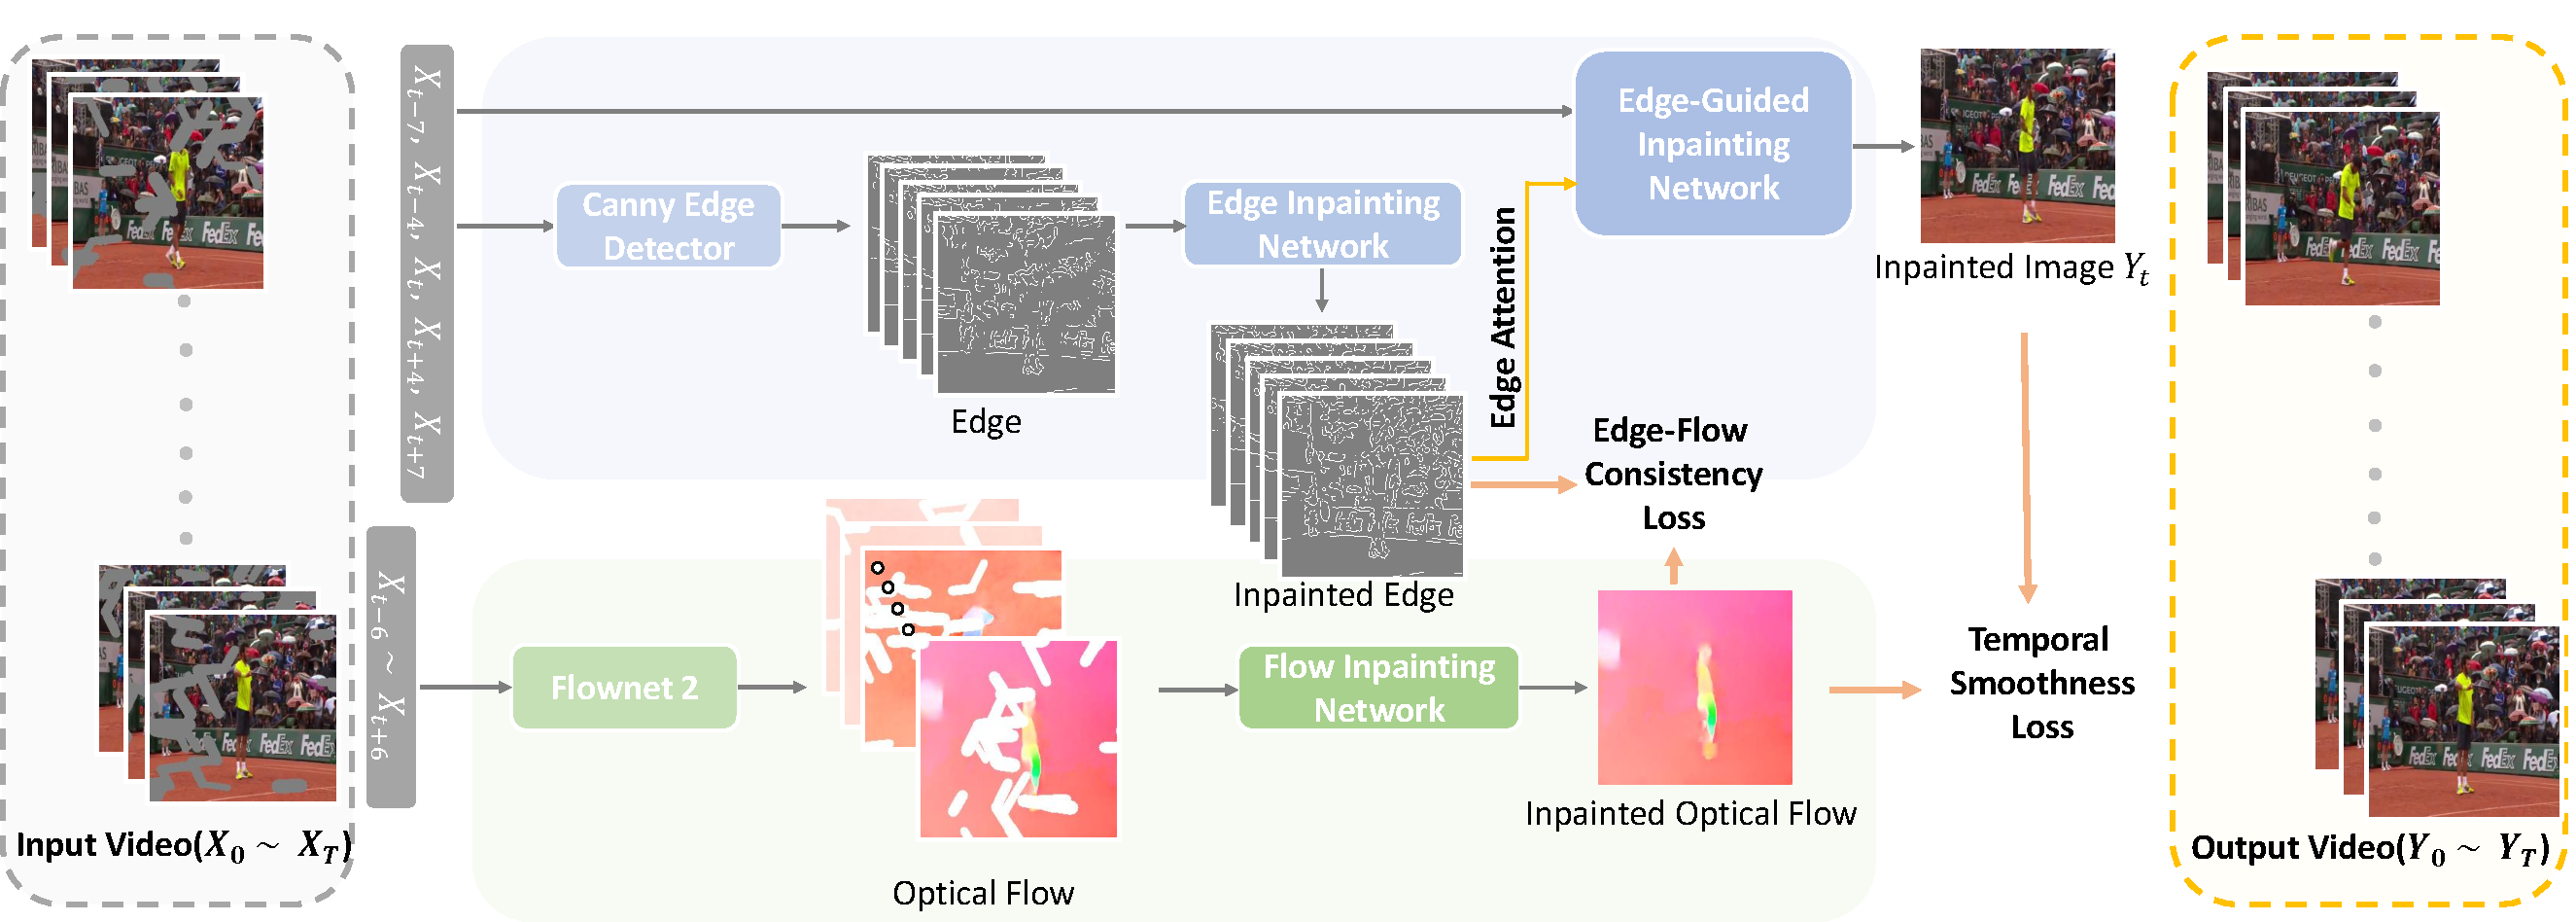
\includegraphics[width=1.0\columnwidth]{zong} % Reduce the figure size so that it is slightly narrower than the column. Don't use precise values for figure width.This setup will avoid overfull boxes. 
	\caption{Overview of our structure-guided inpainting network. We first completes the missing edges by aggregating information from neighboring frames to represent target structure using the ENet. Then, the TexNet synthesizes textures under the structure guidance. Moreover, the FNet is designed to predict missing optical flow to enforce temporal coherence.}
	\label{zong}
\end{figure}


In traditional studies of video inpainting, a common formulation is patch-based composition by exploiting complementary information across neighboring frames and compositing visually pleasing content in the missing regions via patches~\cite{patwardhan2007video,wexler2004space,newson2014video}.
% 
The inpainting quality of these methods strongly relies on the hypothesis that the missing content in the corrupted region appears in neighboring frames, which limits their generalization.
%
Recently, deep-learning-based methods achieve great performance improvement.
A straightforward solution is to utilize 3D convolution layers to extract spatiotemporal features and predict missing content with smooth motion \cite{wang2019video}.
Optical flow is commonly used in subsequent methods to aggregate contextual information from neighboring frames and synthesize temporally smooth results~\cite{Xu_2019_CVPR,Kim_2019_CVPR,Kim_2019_CVPR1}.
%
By introducing motion guidance, these methods pay more attention on temporal smoothness, however, structure rationality and object details have not been well explored. 
%However, structural rationality is also a significant factor for realistic video inpainting. 
%
Without definite representation and generation of the target structure, these methods tend to produce over-smoothed regions. 
Similar observations has been obtained in image inpainting \cite{Xiong_2019_CVPR,nazeri2019edgeconnect}. %\cite{iizuka2017globally,liu2018partialinpainting,yu2018free}. 
To solve this problem, they propose to predict object contours or edges as auxiliary information to guide texture synthesis.
%
On the other hand, human eyes are sensitive to the temporal discontinuity, which frequently occurs at edges. 
This brings the difficulty of simultaneously completing structure in fine details and preserving temporal coherence in video inpainting.
 
\begin{figure*}[ht]
	\centering
	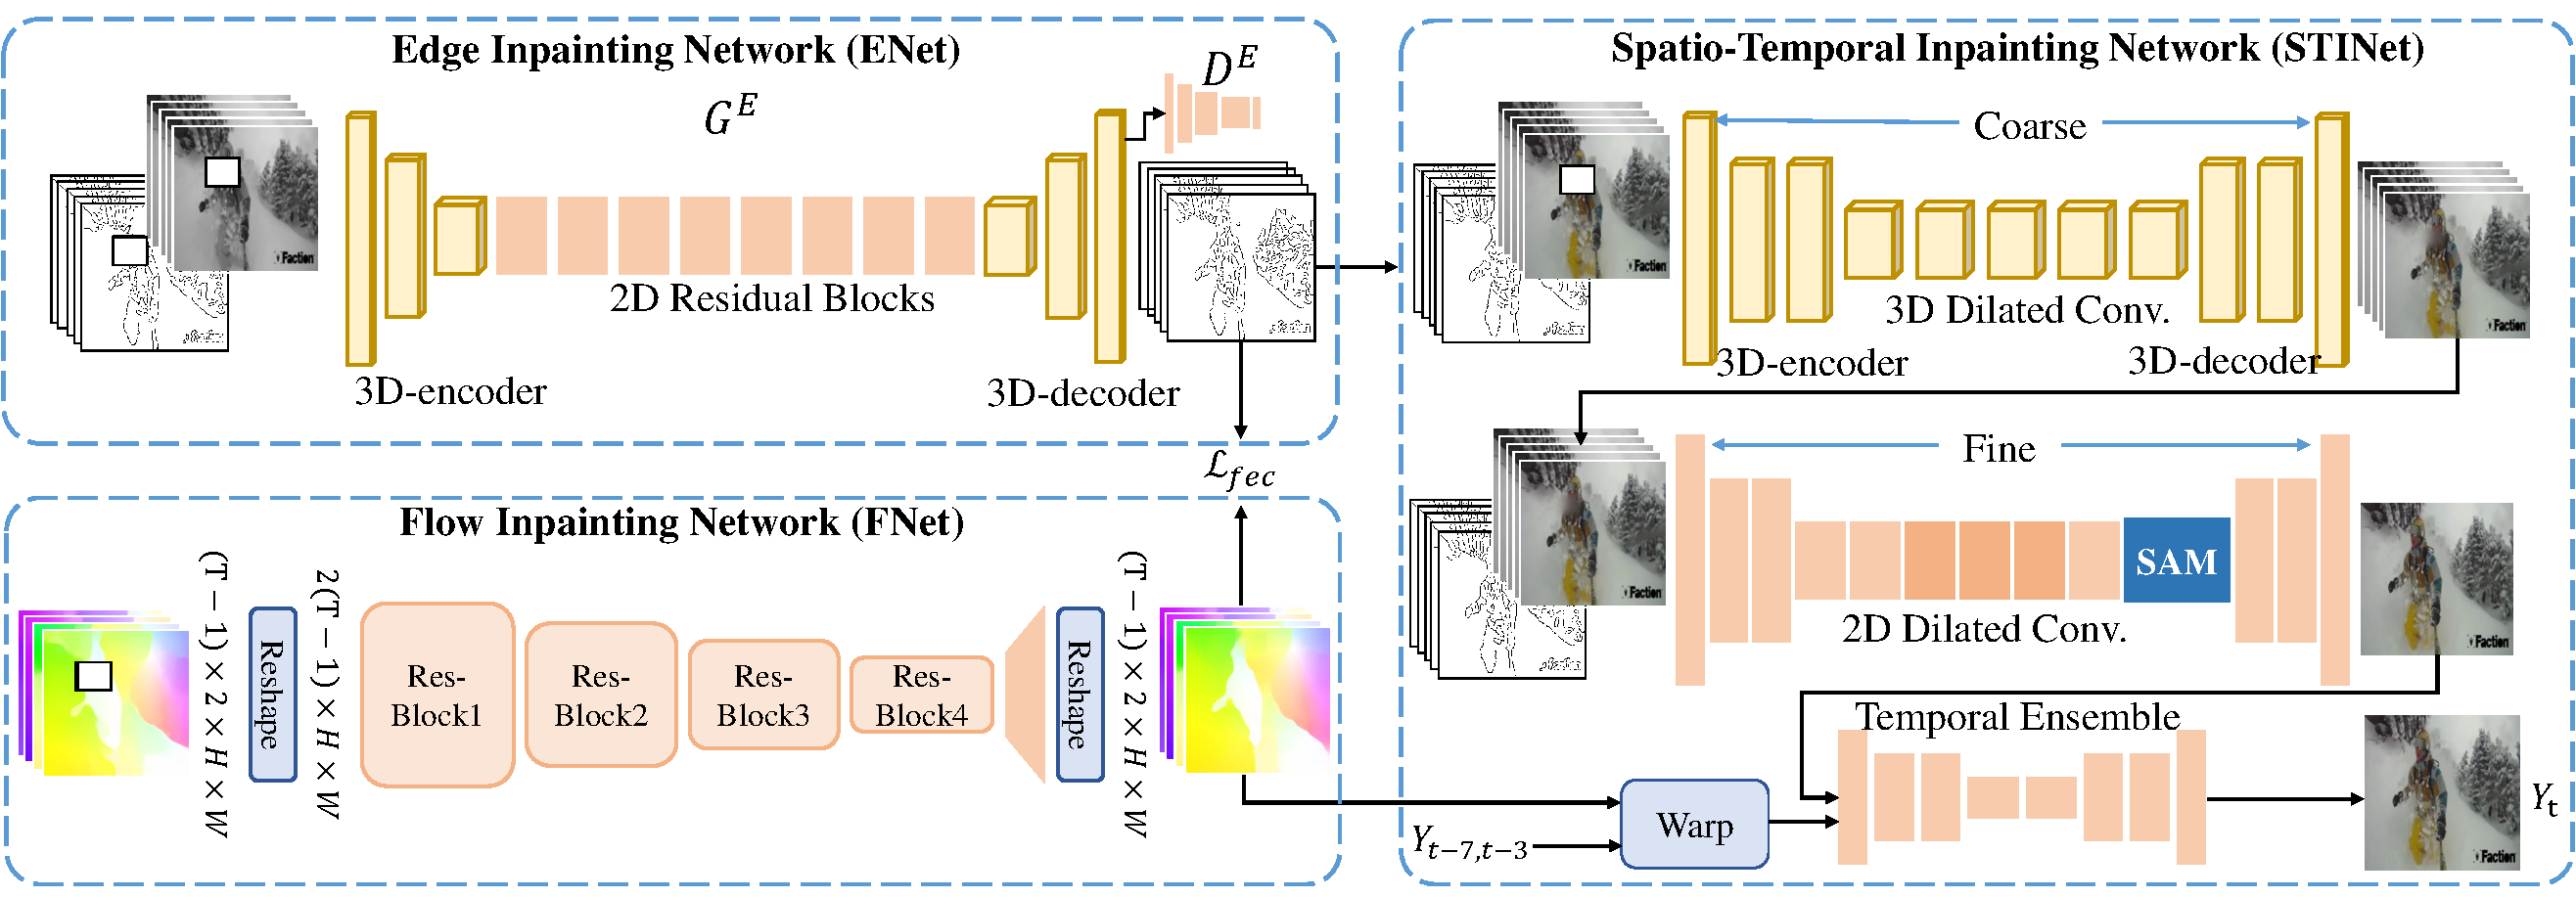
\includegraphics[width=2.0\columnwidth]{sti} % Reduce the figure size so that it is slightly narrower than the column. Don't use precise values for figure width.This setup will avoid overfull boxes. 
	\caption{The detailed architecture of our network. ENet adopts an encoder-decoder architecture to complete edges in the missing regions. TexNet utilizes a coarse-to-fine manner to inpaint the final frames. FNet predicts flows between adjacent frames for flow warping loss and temporal ensemble. }
	%FNet is based on the backbone Resnet-101, which is associated with ENet.
	
	\label{fig:stiNet}
\end{figure*}

In this paper, we present a novel structure-guided video inpainting approach that effectively exploits the spatio-temporal structure information to improve video inpainting quality.  
We explore the correlation among structure, motion, and texture in video inpainting to complete the missing region with valid structure, rich visual details, and temporal coherence simultaneously.
%
To synthesize the missing content, we first predict sparse edges that effectively represent the target structure, and then fill textures under the guidance of the concise structure in a coarse-to-fine manner.
To further enhance the temporal coherence of synthesized frames, we employ motion flows to warp neighboring frames to consistency check and temporal ensemble. 



As shown in Fig.~\ref{zong}, our method consists of three modules, which are respectively an edge inpainting network (ENet), a texture inpainting network (TexNet), and a flow inpainting network (FNet).
%
Given multiple adjacent frames with masks, ENet first completes edge maps that depict the target structure. 
Then, under the guidance of the completed edges, TexNet fills the pixel colors and textures in a coarse-to-fine manner.
A structure attention module is designed to capture the latent spatial relevance between video textures and edges.
Compared with original edge maps, the structure-texture relevance is more efficiently embedded in TexNet, which benefits fine-detailed frame generation.
Besides, the developed FNet predicts the missing optical flow, which provides auxiliary motion knowledge. 
Explicitly, a flow-edge consistency constraint and a temporal ensemble module are utilized to smoothen the edge maps and final inpainted frames. 
Consequently, the inpainted frames using our approach are not only temporal consistent, but also complete in structure and rich in visual details.
 

%In summary, we present a novel structure-guided video inpainting method, which can generate structural reasonable and temporal coherent inpainted frames.
%
Experiments on the YouTubeVOS and DAVIS datasets show that the proposed method obtains new state-of-the-art performance with low time consumption.
%
Our technical contributions can be summarized as follows:
\begin{itemize}
	\item We propose a novel structure-guided video inpainting method, which combines edge completion, flow estimation, and realistic texture inpainting for synthesizing missing content with fine details and temporal consistency.
	\item A structure attention module is designed to capture the correlation between appearance and structure and provide more effective structural guidance to texture synthesis.
	\item A flow-guided warping and temporal ensemble module are developed to enhance the temporal consistency of both completed edges and video frames.   
\end{itemize}





\section{Related Work}
\paragraph{Traditional Image/Video Inpainting.}
Traditional methods of image and video inpainting can be divided into two categories, diffusion-based and patch-based methods. 
Diffusion-based methods \cite{bertalmio2000image,ballester2001filling} gradually propagate contents from surrounding areas to the missing region. 
However, this kind of method fails to handle large holes due to its assumption of local smoothness. 
%
Patch-based methods~\cite{bertalmio2003simultaneous,efros2001image}, which are more widely used, formulate the completion task as a patch-based optimization problem. 
This type of method fills the missing content by borrowing and aggregating the most similar patches from known regions. 
%
For video inpainting, a series of methods have been proposed by searching patches across frames~\cite{patwardhan2007video}, extending the 2D PatchMatch algorithm~\cite{barnes2009patchmatch} to improve inpainting quality \cite{newson2014video}, or jointly estimating optical flow and colors to promote temporal coherence \cite{huang2016temporally}. 
%However, traditional methods assume that there exist similar contents in known regions, thus fail to synthesize unseen appearances. 
However, the propagation process makes these methods suffer from high computational complexity, which limits their usage in practical applications. 

\paragraph{CNN-based Image Inpainting.}
Recently, deep learning methods have achieved tremendous progress in image and video inpainting because of their capability of capturing high-level semantic information of images and videos. 
%
The convolution neural network (CNN) is first introduced for image denoising and inpainting in \cite{xie2012image}. 
To improve the photorealism of the completed results, a generative adversarial network is employed \cite{pathak2016context}.
%by jointly training a generator and a discriminator in a minimax manner. 
Multiple discriminators can be used to constrain both global and local coherence of image contents \cite{iizuka2017globally}. 
Subsequent approaches solve more specific problems in image inpainting, such as inpainting irregular holes with partial convolution~\cite{liu2018partialinpainting} and gated convolution \cite{yu2018free} for dynamic feature selection.
%
\mdf{While these methods tend to generate over-smoothed and blurry results, a two-stage approach is proposed to hallucinate edges first and then fill pixel colors using the edges as a prior \cite{nazeri2019edgeconnect}.}
\mdf{Though high quality static images with reasonable structure can be generated using this method, simply extending it from image to video by 3D convolutions inevitably fails because of no guarantee on the temporal coherence.}
%These image inpainting methods can obtain plausible synthesized images. 
%\cite{nazeri2019edgeconnect} introduces an edge generator to refine generated structure in image inpainting. 
 

%%% video inpainting 
\paragraph{Deep Video Inpainting.}
%However, directly extending these state-of-the-art image inpainting methods to video domain is not an optimal solution, which will generate videos with serious temporal flickers, artifacts and jitters. 
Besides of the challenge in maintaining temporal coherence, image inpainting methods do not fully utilize useful complementary information in neighboring frames, which could help large hole completion.
Several methods based on deep neural networks have been proposed just recently.
%
The first CNN-based video inpainting method is CombCN \cite{wang2019video}, which jointly learns temporal structure and spatial details via 3D convolutions.
%%\cite{Xu_2019_CVPR} proposes a stacked convolution network to predict missing motion field and regards video inpainting as a pixel propagation problem. 
%
To enforce temporal coherence, a recurrent feedback is employed to connect consecutive frames~\cite{Kim_2019_CVPR,Kim_2019_CVPR1}. 
Instead of filling pixel colors directly using CNNs, a deep flow completion network is proposed to propagate pixel colors based on the estimated flow in the missing region~\cite{Xu_2019_CVPR}.
%
However, these existing methods neglect the importance of intact structure in video inpainting and typically suffer from blurs and structural cracks in the synthesized frames.  
In comparison, we propose to explicitly complete the target structure using edges, which are efficient to predict due to their sparsity. 
Under the structural guidance, more pleasing results could be synthesized with reasonable structure and fine details. 

%Different from the methods above, we extract and refine structure information explicitly, which will generate fine-detailed video inpainting results.

%\cite{Kim_2019_CVPR} automatically removes texts in videos without mask indications, which aggregates temporal features from encoder to decoder and applies a recurrent feedback. 
%\cite{Kim_2019_CVPR1} introduces convolutional LSTM and temporal feature aggregation to obtain temporal consistency and learn information from neighboring frames. 
 


 
























